\chapter{Rossby Modes in the Solar Mean Magnetic Field}\label{chap:rmode}

%%%%%%%%%%%%%%%%%%%%%%%%%%%%%%%%%%%%%%%%%%%%%%%%%%%%%%%%%%%%%%%%%%%%%
%%%%%%%%%%%%%%%%%%%%%%%%%%%%%%%%%%%%%%%%%%%%%%%%%%%%%%%%%%%%%%%%%%%%%
\section{Introduction}\label{sec:rmode_intro}


Rossby waves, as first derived by \citet{rossby_relation_1939}, have recently been discovered in the Sun through observations of near-surface flows by the \gls{sdo/hmi} \citep{loptien_global-scale_2018, liang_time-distance_2019}.

Standing Rossby waves, or $r$ modes, are toroidal modes of oscillation of a rotating, fluid body for which the dominant restoring force against the pressure gradients is the Coriolis force \citep{lanza_sectoral_2019, hathaway_hydrodynamic_2020}. Rossby waves are associated with an undulation of a flow resulting in a pattern of radial vorticity of alternating sign. They are understood to form in the high atmosphere on Earth, heavily influencing global weather. For the Sun we observe that Rossby waves propagate in the retrograde direction, in the Carrington reference frame.

Recently, \citet{loptien_global-scale_2018} provided an unambiguous detection of sectoral solar $r$ modes by tracking the horizontal flows of granules in the solar photosphere during a 6-year period, using observations by \gls{sdo/hmi}. Following this study \citet{liang_time-distance_2019} confirmed the detection of solar $r$ modes with time-distance helioseismology to measure deeper, subsurface flows in the meridional direction along the solar equator using both \gls{soho/mdi} and \gls{sdo/hmi} data, covering 21 years. In addition, \citet{hanasoge_detection_2019} were also able to show the detection of solar $r$ modes using a normal-mode coupling technique on 2 years of \gls{sdo/hmi} data. In both of the observation conducted by \citet{loptien_global-scale_2018} and \citet{liang_time-distance_2019}, the average lifetime of the $r$ modes were on the order of several months, and as long as a over a year for specific modes.

By monitoring the proper motions of solar supergranules using a local correlation tracking method \citet{hathaway_hydrodynamic_2020} also report observing low latitude Rossby waves in full-disk Doppler images obtained by \gls{sdo/hmi}, extending the measurements of Rossby waves to greater depths in the solar atmosphere, by an order of magnitude. The $r$ modes observed using the supergranules have lifetimes which are only slightly longer than the Carrington rotation period, hence in slight disagreement with \citet{loptien_global-scale_2018} and \citet{liang_time-distance_2019}, which \citet{hathaway_hydrodynamic_2020} claim may be due the waves getting in and out of phase with each other as the low wave number waves propagate faster than the higher wave number waves. As these observations are at low latitudes, it is possible that they are linked to active magnetic regions and hence could be manifested in other sources of magnetic data.

Here we present the search for evidence of a magnetic signature of the global $r$ modes using 21 years of \gls{bison} observations of the \gls{los} \gls{smmf} (for details on the \gls{smmf} and \gls{bison}, see \citet{chaplin_studies_2003} and references within).

In an earlier study of the \gls{smmf}, the power spectrum of the \gls{bison} observations was modelled using a combination of Lorentzian peaks and a convolution with the window function to account for the effect of gaps in the data. The full spectrum and the fit are shown in Figure~\ref{fig:BiSON_PSD}.

%\begin{figure}[!ht]
%	\centering
%	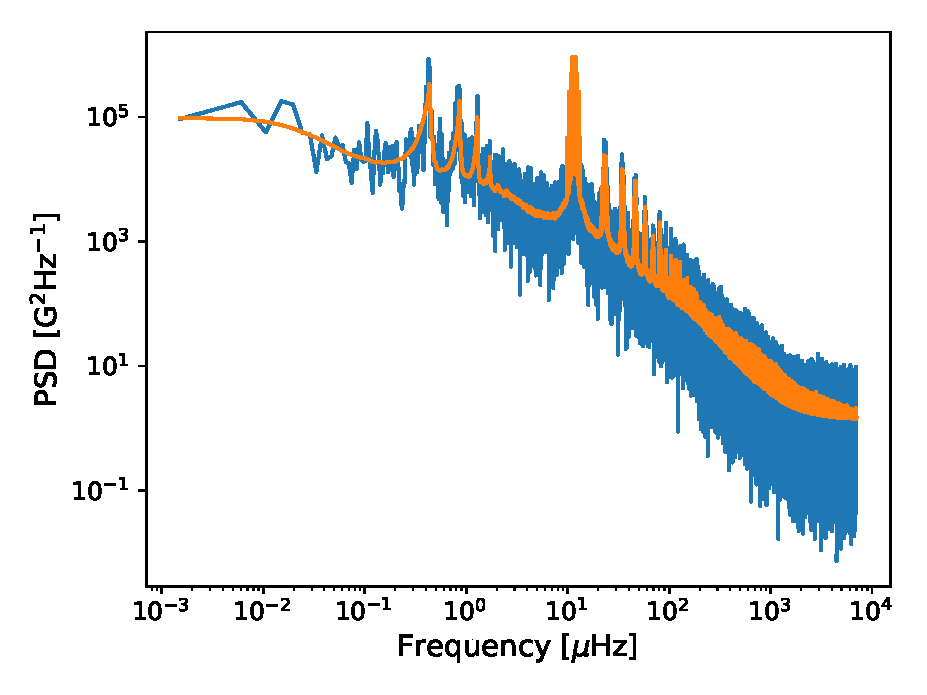
\includegraphics[width=0.7\columnwidth]{SMMF_PSD_fit.eps}
%	\caption{Model fit to the full BiSON SMMF PSD.}
%	\label{fig:BiSON_PSD}
%\end{figure}


\begin{figure}[ht!]
	\centering
	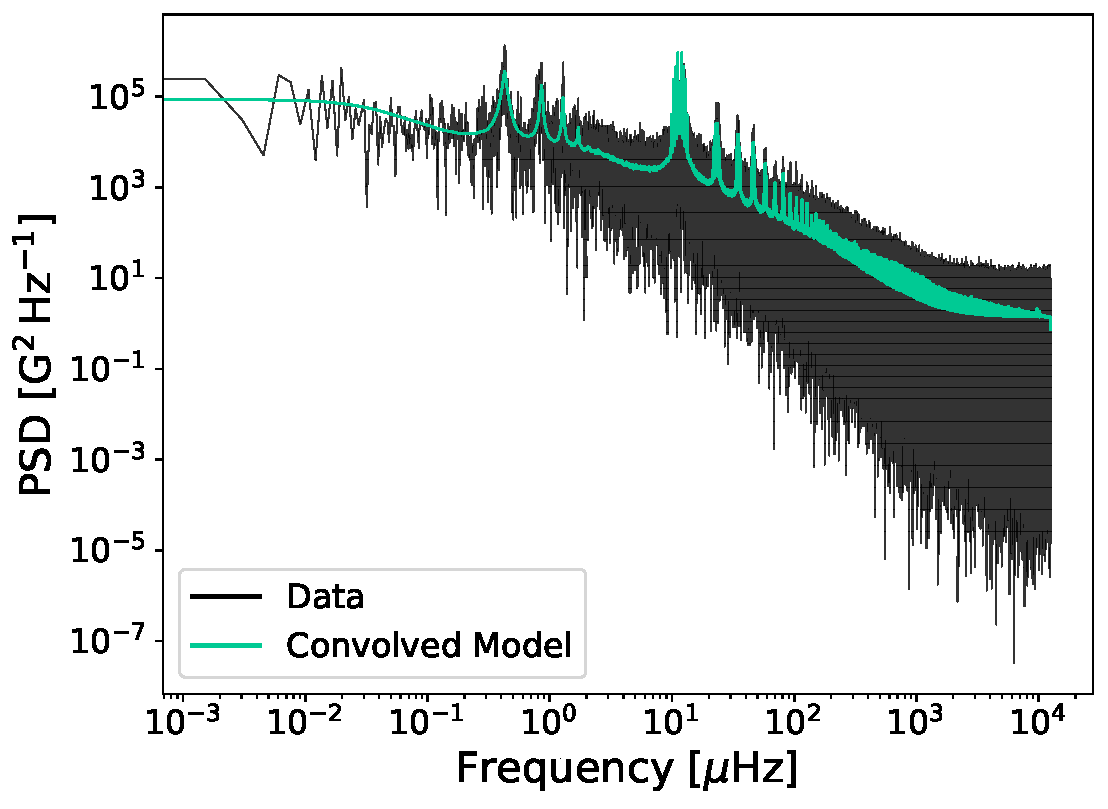
\includegraphics[width=\columnwidth]{BiSON_PSD_model.pdf}
	\caption{Full, modelled power spectrum of the BiSON SMMF on logarithmic axes. The data is displayed in black and the convolved model using asymmetric Lorentzian peaks is shown in green.}
	\label{fig:BiSON_PSD}
\end{figure}

We can divide through by the model, to achieve the residual spectrum, in which we have searched for the magnetic signatures of $r$ modes. %We find that although there exists a promising narrow-band region of significant power in the \gls{bison} residuals spectrum, which could be the $l=m=2$ mode, the $r$ mode does not exist in other sources of \gls{smmf} data, hence the observed peak is more likely explained as being a source of prominent noise in the \gls{bison} observations.

Further analysis was also performed using simulated data to better understand how an annual modulation of observations would affect the $r$-mode frequencies.


%%%%%%%%%%%%%%%%%%%%%%%%%%%%%%%%%%%%%%%%%%%%%%%%%%%%%%%%%%%%%%%%%%%%%%
%%%%%%%%%%%%%%%%%%%%%%%%%%%%%%%%%%%%%%%%%%%%%%%%%%%%%%%%%%%%%%%%%%%%%%
%\section{Aims}\label{sec:r-mode_aims}
%
%In this chapter the residual power spectrum of the \gls{bison} \gls{smmf}, after removing a model for the dominant signal, was investigated in order to search for the existence of $r$ modes. Within the residual spectrum we test for the existence of $r$ modes and where they appear to exist, a Lorentzian model is fit to the peak to understand the properties of the source.
%
%Further analysis is provided using simulated data to better understand how an annual modulation of the $r$ mode observations would affect their frequencies. In addition, \gls{sdo/hmi} data are investigated to support the argument that $r$ modes are not split in the power spectrum and instead we should observe the central mode frequency and lower amplitude side bands.



%%%%%%%%%%%%%%%%%%%%%%%%%%%%%%%%%%%%%%%%%%%%%%%%%%%%%%%%%%%%%%%%%%%%%
%%%%%%%%%%%%%%%%%%%%%%%%%%%%%%%%%%%%%%%%%%%%%%%%%%%%%%%%%%%%%%%%%%%%%
\section{Theory}\label{sec:r-mode_theory}

The detailed theory of the effect of $r$ modes on observational data was re-visited recently by \citet{lanza_sectoral_2019} in light of the solar observations, in an effort to determine the effect of the $r$ modes on radial velocity detections of exoplanets.

Under the assumption of a slow, uniformly rotating sphere (with angular velocity, $\Omega$, where $\Omega^2 << GMR^{-3}$), the frequencies of global $r$ modes in the Carrington rotating frame is well approximated by equation~(\ref{eq:dispersion_rel}), where $l > 0$ is the angular degree and $m$ is the azimuthal order \citep{loptien_global-scale_2018, lanza_sectoral_2019}:

\begin{equation}
\nu_{carr} = - \frac{2m\Omega}{l(l + 1)} \, .
\label{eq:dispersion_rel}
\end{equation}

In an inertial frame the observed $r$ mode frequencies will be \citep{lanza_sectoral_2019}:

\begin{equation}
\nu_{\mathrm{in}}(l,m) \approx m\Omega - \frac{2m\Omega}{l(l + 1)}  = m\Omega \left(1 - \frac{2}{l(l + 1)}\right) \, ,
\label{eq:r-mode}
\end{equation}

where $\Omega$ is the mean sidereal rotation rate, and $l$ and $m$ are the angular and azimuthal degree, respectively. Sectoral Rossby waves are obtained by setting $l=m$ in this equation. A consequence is that they propagate with a retrograde phase velocity as $\nu / m = -2 \Omega/[m(m + 1)] < 0$.

An Earth-based observer, orbiting the sun, shall expect to observe frequencies adjusted by the orbital frequency, $\nu_\oplus \, \approx \, 31.7$nHz, given by equation~(\ref{eq:r-mode_obs}):

\begin{equation}
\nu_{\mathrm{obs}}(l,m) = \nu_{\mathrm{in}}(l,m) - m\nu_{\oplus} \, .
\label{eq:r-mode_obs}
\end{equation}

In addition, due to the tilt of the ecliptic with respect to the solar equatorial plane (the solar $B_0$ angle), the visibility of the modes will vary on a timescale of 1 year, meaning we expect to actually observe split peaks at frequencies of $\nu_{\mathrm{obs}}(l,m) \pm \nu_{\oplus}$ \citep{lanza_sectoral_2019}).

Based on this theory, we can predict the the frequencies at which to search for $r$ modes. These frequencies are summarised in Table~\ref{tab:r-modes}, along with the frequencies observed in other studies. %compare the observed sectoral $r$ modes with those predicted. These frequencies are summarised in Table~\ref{tab:r-modes}.

\begin{table}[ht!]
	\begin{center}
		\caption{Predicted$^+$ and observed$^\circ$ $r$ mode frequencies for combinations of $l$ and $m$. Predicted frequencies and conversions of observations to different frames of reference use equation~(\ref{eq:dispersion_rel}), equation~(\ref{eq:r-mode}), and equation~(\ref{eq:r-mode_obs}), with $\Omega = 453.1$ nHz. The predicted splitting for the $B_0$ angle variation is also provided. The key for the source column is: LPT for \citet{loptien_global-scale_2018}, LNG for \citet{liang_time-distance_2019}, and LZA for \citet{lanza_sectoral_2019}.}\label{tab:r-modes}
		\begin{tabular}{c c c c c c }
			\hline 
			{\bf Frequency } & {\bf Source} & {\boldmath$l=m=2$} & {\boldmath$l=m=3$} & {\boldmath$l=m=4$} & {\boldmath$l=m=5$}  \\ 
			\hline 
			& LPT$^\circ$ & -- & -259 & -194 & -157 \\ 
			$\nu_{carr} \, [nHz]$ & LNG$^\circ$ & -- & -253 & -198 & -156 \\ 
			& LZA$^+$ & --302.1 & -226.6 & -181.2 & -151.0 \\ 		
			\hline 
			
			& LPT & -- & 1100 & 1618 & 2109 \\ 
			$\nu_{in} \, [nHz]$  & LNG & -- & 1106 & 1614 & 2110 \\ 
			& LZA & 604.1 & 1132.8 & 1631.2 & 2114.5 \\ 		
			\hline 
			
			& LPT & -- & 1005.2 & 1491.7 & 1950.1 \\
			$\nu_{obs} \, [nHz]$ & LNG & -- & 1011.2 & 1487.7 & 1951.1 \\
			& LZA & 540.8 & 1037.7 & 1504.4 & 1956.0 \\ 
			\hline 		
			
			& LPT &  -- & 1036.9 & 1523.3 & 1981.8 \\ 
			$\nu_{obs} + \nu_{\oplus} \, [nHz]$ & LNG & -- & 1042.9 & 1519.3 & 1982.8 \\ 
			& LZA & 572.4 & 1069.4 & 1536.1 & 1987.7 \\ 
			\hline 
			
			& LPT & -- & 973.6 & 1460.0 & 1918.4 \\   
			$\nu_{obs} - \nu_{\oplus} \, [nHz]$ & LNG & -- & 979.6 & 1456.0 & 1919.4 \\  
			& LZA & 509.1 & 1006.0 & 1472.7 & 1924.3 \\ 
			\hline 
			
		\end{tabular} 
	\end{center}
\end{table}




%%%%%%%%%%%%%%%%%%%%%%%%%%%%%%%%%%%%%%%%%%%%%%%%%%%%%%%%%%%%%%%%%%%%%
%%%%%%%%%%%%%%%%%%%%%%%%%%%%%%%%%%%%%%%%%%%%%%%%%%%%%%%%%%%%%%%%%%%%%
\section{Methodology}\label{sec:r-mode_method}

\subsection{Testing the Residual Spectrum}
In order to investigate the presence of Rossby wave modes in the power spectrum of the \gls{bison} \gls{smmf}, statistical significance tests were employed using a false-alarm approach, to test the probability of finding prominent narrow-band power in the residual spectrum.

We assume negative exponential statistics (i.e. $\chi^2$ 2-degrees of freedom distribution), and that the bins in the power spectrum are uncorrelated. This was tested using artificial data created with the same window function as the BiSON observations, and we showed that this assumption was suitable. We then calculated the false alarm probability, or probability to observe power in a given frequency bin, $\nu$, that is greater than or equal to a given threshold. The probability to observe power in a given frequency bin, $\nu$, that is greater than or equal to $P(\nu)$ is:

\begin{equation}
p[P(\nu)] = \frac{1}{P_{lim}(\nu)} \mathrm{exp}\left(-\frac{P(\nu)}{P_{lim}(\nu)}\right) \; \mathrm{or; } \; p[P(\nu)] = \frac{1}{\langle P(\nu) \rangle} \mathrm{exp}\left(-\frac{P(\nu)}{\langle P(\nu) \rangle}\right) \, ,
\label{eq:p_power_prob}
\end{equation}


where $P_{lim}(\nu)$ is the limit spectrum or $\langle P(\nu) \rangle$ is a well-fitting model/estimate to the spectrum. Considering a relative power approach (i.e. considering the power relative to the mean level or model of the \gls{psd}), equation~(\ref{eq:p_power_prob}) may be written more concisely as:

\begin{equation}
p(s_{\nu}) = e^{(-s_{\nu})} \, ,
\label{eq:p_power_prob_concise}
\end{equation}

where,

\begin{equation}
s_{\nu} = P(\nu)/\langle P(\nu) \rangle \, ,
\label{eq:s_v}
\end{equation}

and $\langle P(\nu) \rangle$ is reduced to 1 when we compare the power relative to the power spectrum residuals.

In reality, we used the $\chi^2$ cumulative distribution function to compute the probability of power, which is given by equation~(\ref{eq:chi2_CDF}), where $k$ is the number of degrees of freedom, $\gamma(s,t)$ is the lower incomplete gamma function and $P(s,t)$ is the regularized gamma function: 

\begin{equation}
F(x; \, k) = \frac{\gamma (\frac{k}{2}, \, \frac{x}{2})}{\Gamma(\frac{k}{2})} = P\left(\frac{k}{2}, \, \frac{x}{2}\right) \, .
\label{eq:chi2_CDF}
\end{equation}


Using these expressions, we can rewrite the equation for $P(s_{\nu})$ as given by equation~(\ref{eq:chi2_prob_concise}): 

\begin{equation}
p(s_{\nu}) = 1 \, - \, F(2s_{\nu}; \, k) =1 \, - \, P\left(\frac{k}{2}, \, s_{\nu}\right) \, .
\label{eq:chi2_prob_concise}
\end{equation}

This formulation provided the capability to compute the probability of statistically significant peaks in the residuals for re-binned data, for when data is binned over n-bins, the statistics becomes $\chi^{2}$ with 2n degrees of freedom \citep{appourchaux_detecting_2004}.

The probability that a bin has power at or above the level $s_{\nu}$ is therefore given by equation~(\ref{eq:p_power_prob_concise}), or more generally by equation~(\ref{eq:chi2_prob_concise}), hence the probability that we fail to find a bin with power at or above the level $s_{\nu}$ is $1 \, - \, p(s_{\nu})$; thus the probability of failing to find a bin with power at or above $s_{\nu}$ in $N$-bins in the spectrum is $[1 \, - \, p(s_{\nu})]^N$. Therefore the probability to find at least one bin with power at or above $s_{\nu}$ in N-bins in the spectrum is:

\begin{equation}
p_N = 1\, - \, [1 \, - \, p(s_{\nu})]^N \, ,
\label{eq:p_N}
\end{equation}

where a low value for $p_N$ indicates that the spike in power in that bin is unlikely to be a statistical fluctuation, and therefore is considered a statistically significant spike.

This can be generalised using the cumulative binomial distribution. The probability of finding at least $r$ spikes in $N$-bins at or above the relative power level $s_{\nu}$ is given by equation~(\ref{eq:binom_CDF}), which is equal to equation(\ref{eq:p_N}) when $r=1$,

\begin{equation}
p[r; p(s_\nu), N] = 1 - Pr(X < s_{\nu}) = \sum_{r=r}^{N} \binom{N}{r} \, p(s_{\nu})^r \, [1 \, - \, p(s_{\nu})]^{N-r} \, .
\label{eq:binom_CDF}
\end{equation}

By applying equation~(\ref{eq:binom_CDF}) to the residuals of in the power spectrum, we can test whether there are any significant peaks in the residual power spectrum. Again, a low value for $p[r; p(s_\nu), N]$ indicates that the power in that bin is unlikely to be a statistical fluctuation.


%This can be generalised using the cumulative binomial distribution. The probability of finding at least $r$ spikes in $N$-bins at or above a relative power level, $s_{\nu}$, is given by equation~(\ref{eq:binom_CDF}), where $s_{\nu} = P(\nu)/\langle P(\nu) \rangle$, and $\langle P(\nu) \rangle$ is reduced to 1 when we compare the power relative to this estimate, i.e. the residual PSD.
%
%\begin{equation}
%p[r; p(s_\nu), N] = 1 - Pr(X < s_{\nu}) = \sum_{r=r}^{N} \binom{N}{r} \, p(s_{\nu})^r \, [1 \, - \, p(s_{\nu})]^{N-r}
%\label{eq:binom_CDF}
%\end{equation}
%
%By applying equation~(\ref{eq:binom_CDF}) to the residuals of in the power spectrum, we can test whether there are any significant peaks in the residual power spectrum; a low value for $p[r; p(s_\nu), N]$ indicates that the power in that bin is unlikely to be a statistical fluctuation, and therefore is considered a statistically significant spike.



\subsection{Modelling {\it r} mode Profiles}
In the location of any suspected $r$ modes in the residual spectrum, we can model the profile of the peak by using a Lorentzian distribution, using the form expressed by equation~(\ref{eq:lorentzian}), where $A$ is the amplitude of the signal, $\Gamma$ is the line-width of the distribution, and $\nu_0$ is the central frequency of the distribution:

\begin{equation}
P(\nu) = \frac{2A^2/(\pi \Gamma)}{1 + (2(\nu - \nu_0)/\Gamma)^2} \, .
\label{eq:lorentzian}
\end{equation}

This follows the methodology adopted by \citet{loptien_global-scale_2018} and \citet{liang_time-distance_2019}.

Modelling was performed using the {\verb pymc3 } \gls{nuts} extension to a \gls{hmc} sampling algorithm \citep{salvatier_probabilistic_2016}.



%%%%%%%%%%%%%%%%%%%%%%%%%%%%%%%%%%%%%%%%%%%%%%%%%%%%%%%%%%%%%%%%%%%%%
%%%%%%%%%%%%%%%%%%%%%%%%%%%%%%%%%%%%%%%%%%%%%%%%%%%%%%%%%%%%%%%%%%%%%
\section{Results}\label{sec:r-mode_results}

\subsection{Testing the Residual Spectrum}

The residual spectrum is shown in Figure~\ref{fig:residuals}, with the removed model and locations of $r$ mode frequencies predicted by \citet{lanza_sectoral_2019} over-plotted.

It is clear from Figure~\ref{fig:residuals} that there appears to be a resolved peak of narrow-band power in both the location of the $l=m=2$ $r$ mode and perhaps also the upper B$_0$-variation-modulated $l=m=3$ $r$ mode.

\begin{figure}[!ht]
	\centering
	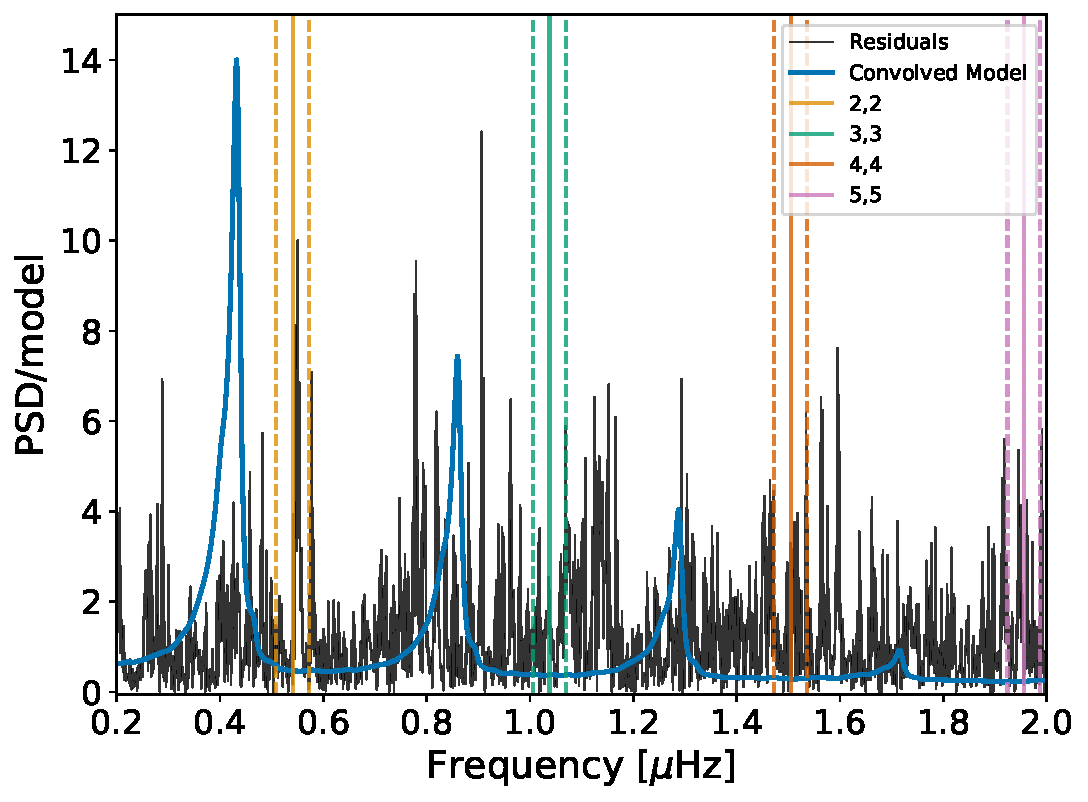
\includegraphics[width=0.65\columnwidth]{asymm_div_r-modes_obs.pdf} 
	\caption{Residual power spectrum of the BiSON SMMF. Over plotted in the green curve is the model of the main SMMF signal. Also over plotted as vertical solid lines are the expected locations of the 4 lowest-frequency sectoral $r$ modes and the dashed lines, the locations of the B$_0$ variation frequency splitting. Dashed lines represent $\pm 31.7$~nHz (i.e. representing the frequencies of splitting due to the variation in the B$_0$ angle.)}  \label{fig:residuals}
\end{figure}

The statistics tests were performed on the residual spectrum for various re-binning factors, n. The plots summarising the statistics tests are shown in Fig.~\ref{fig:BiSON_new_asymm_stats} for re-binning factors of n = 1, 2, 5, and 10.

\begin{figure}[!ht]
	\centering
	\subfloat[No re-binning]{
		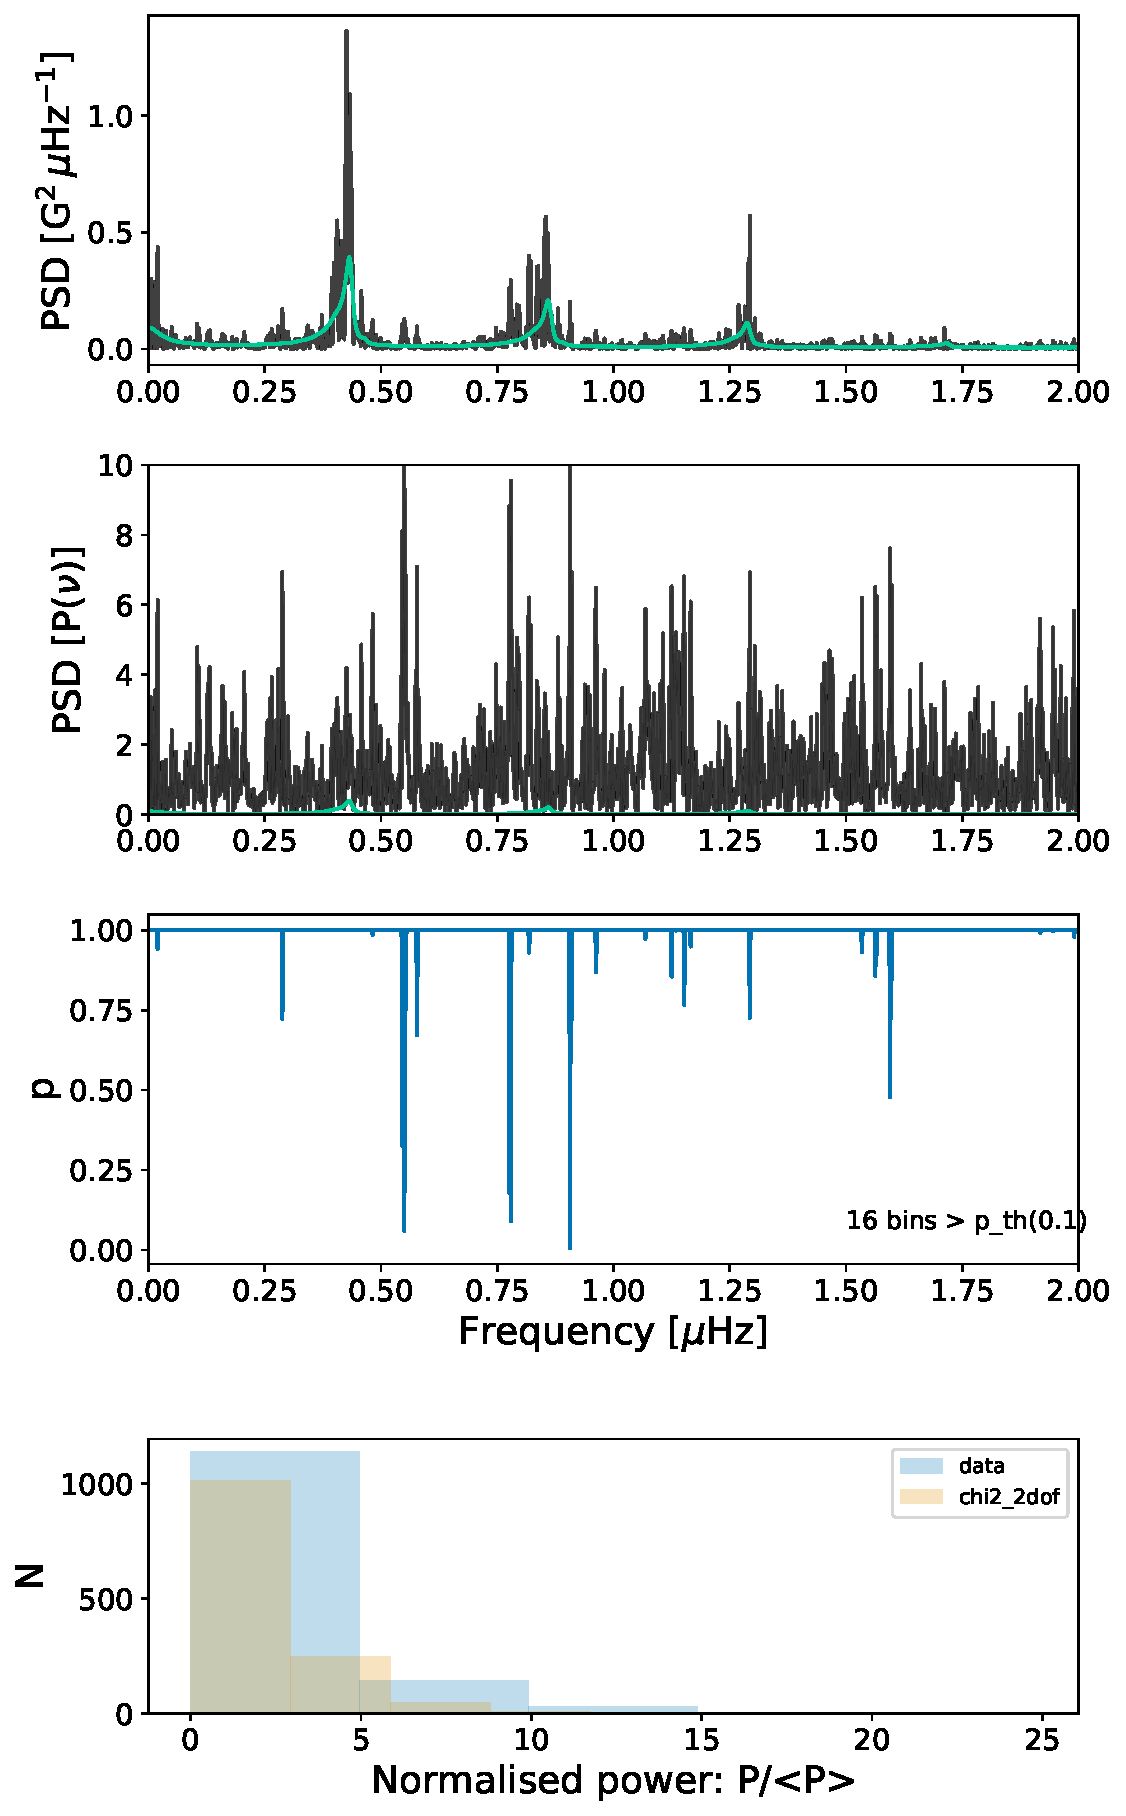
\includegraphics[width=0.35\columnwidth]{full_stats_BiSON_asymm_n1.pdf}
		\label{fig:BiSON_new_asymm_stats_n1}}
	\qquad
	\subfloat[Re-binned by a factor of n=2]{
		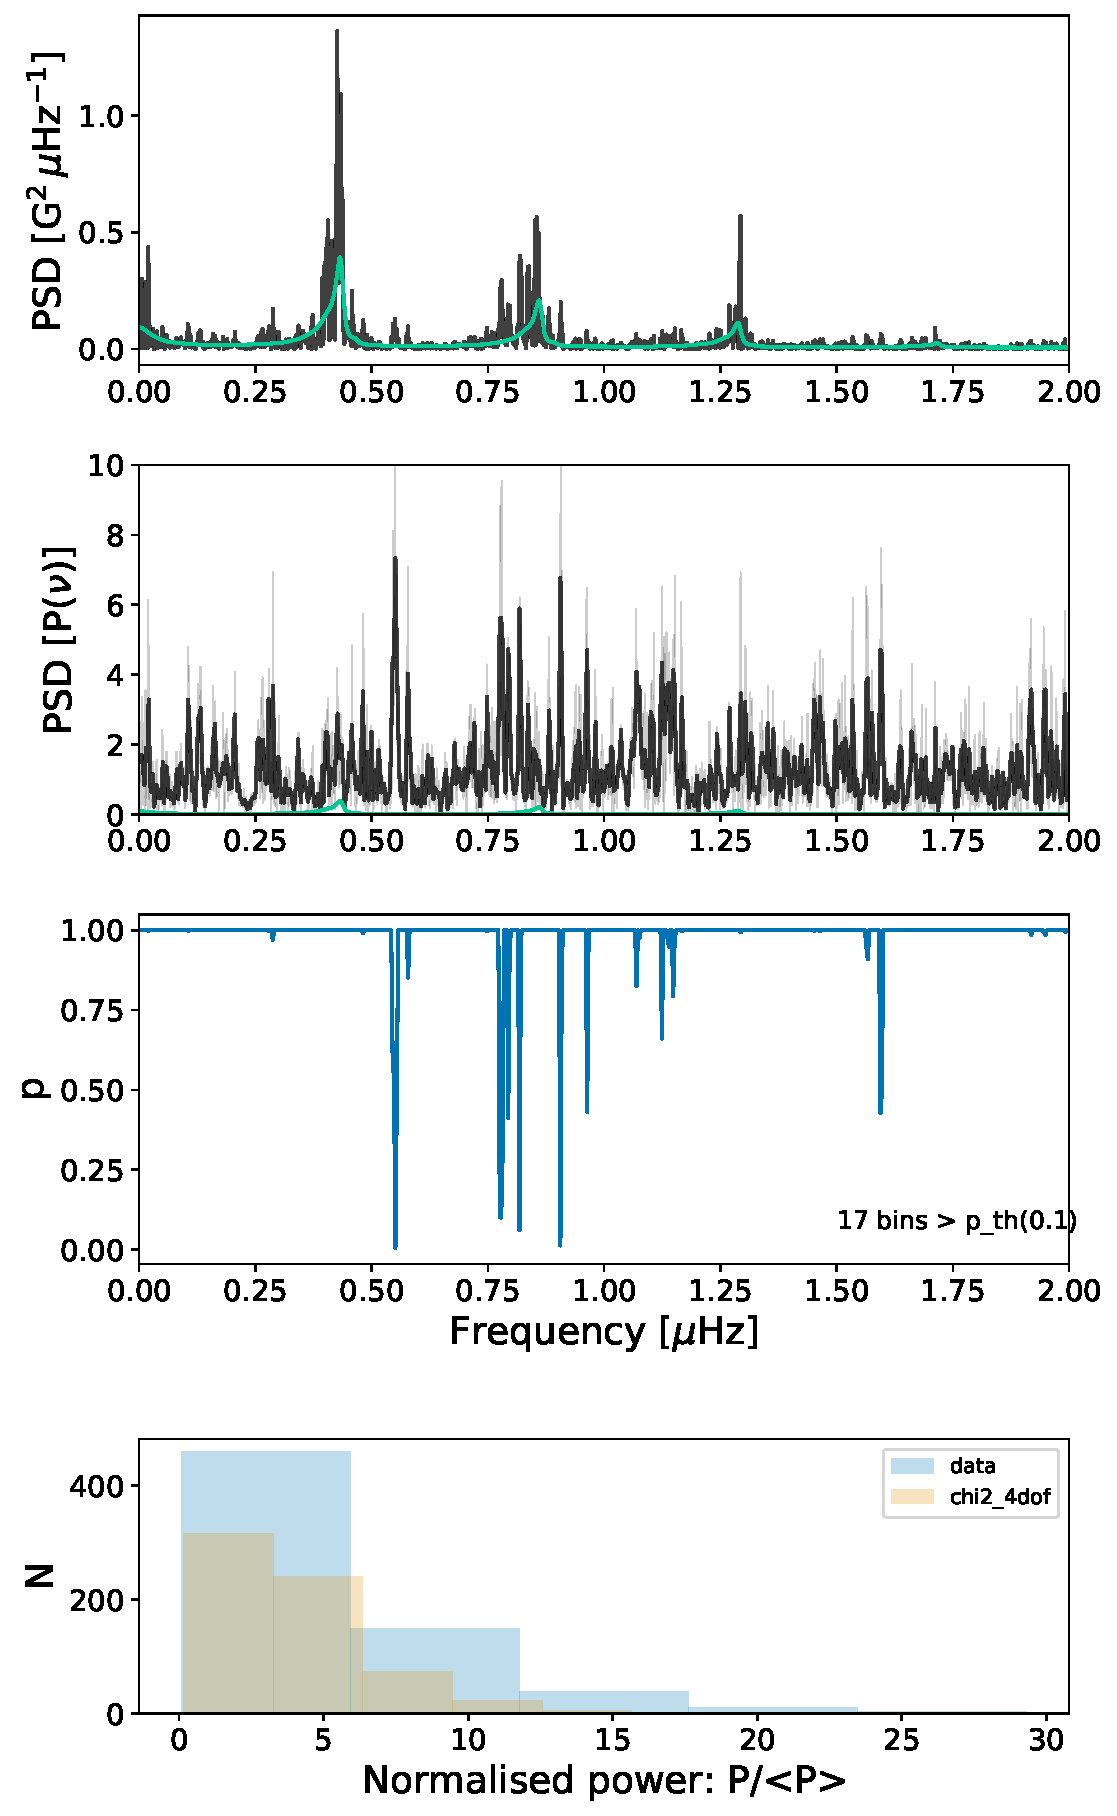
\includegraphics[width=0.35\columnwidth]{full_stats_BiSON_asymm_n2.pdf}
		\label{fig:BiSON_new_asymm_stats_n2}} \\
	
	\qquad
	
	\subfloat[Re-binned by a factor of n=5]{
		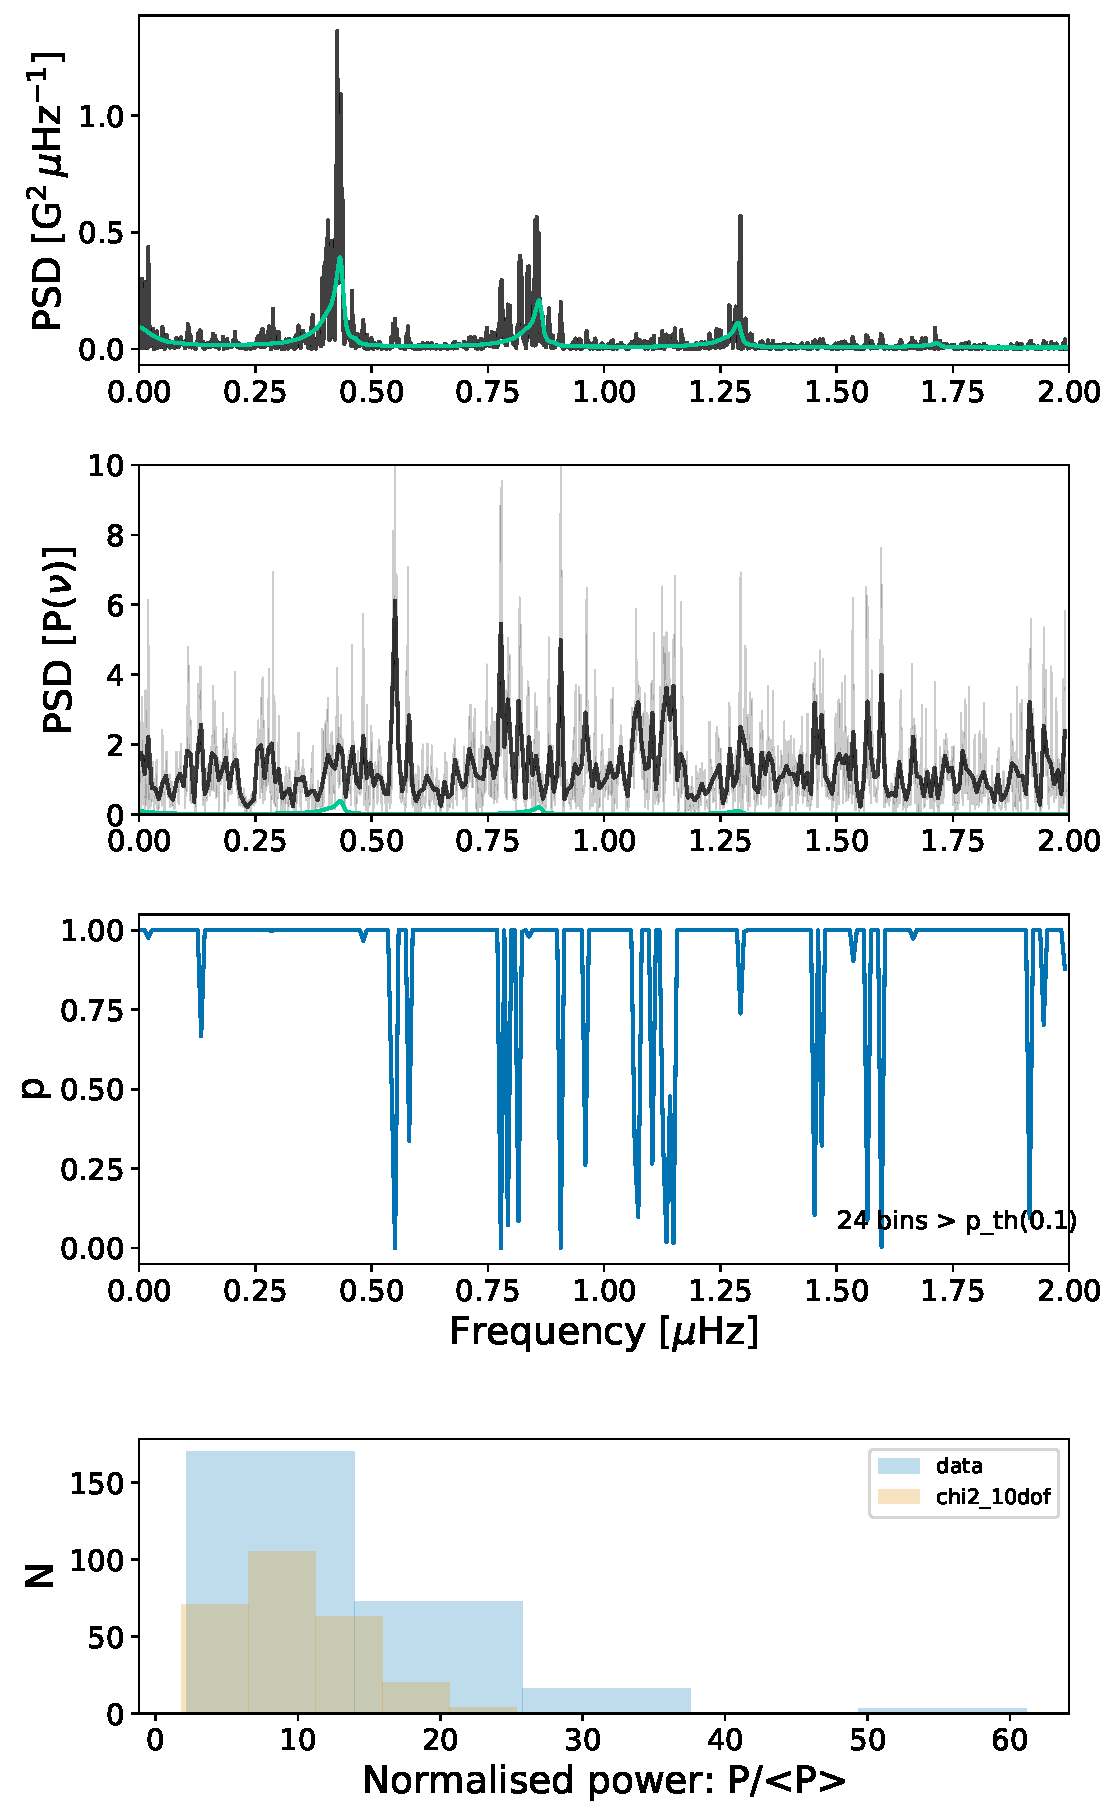
\includegraphics[width=0.35\columnwidth]{full_stats_BiSON_asymm_n5.pdf}
		\label{fig:BiSON_new_asymm_stats_n5}}
	\qquad
	\subfloat[Re-binned by a factor of n=10]{
		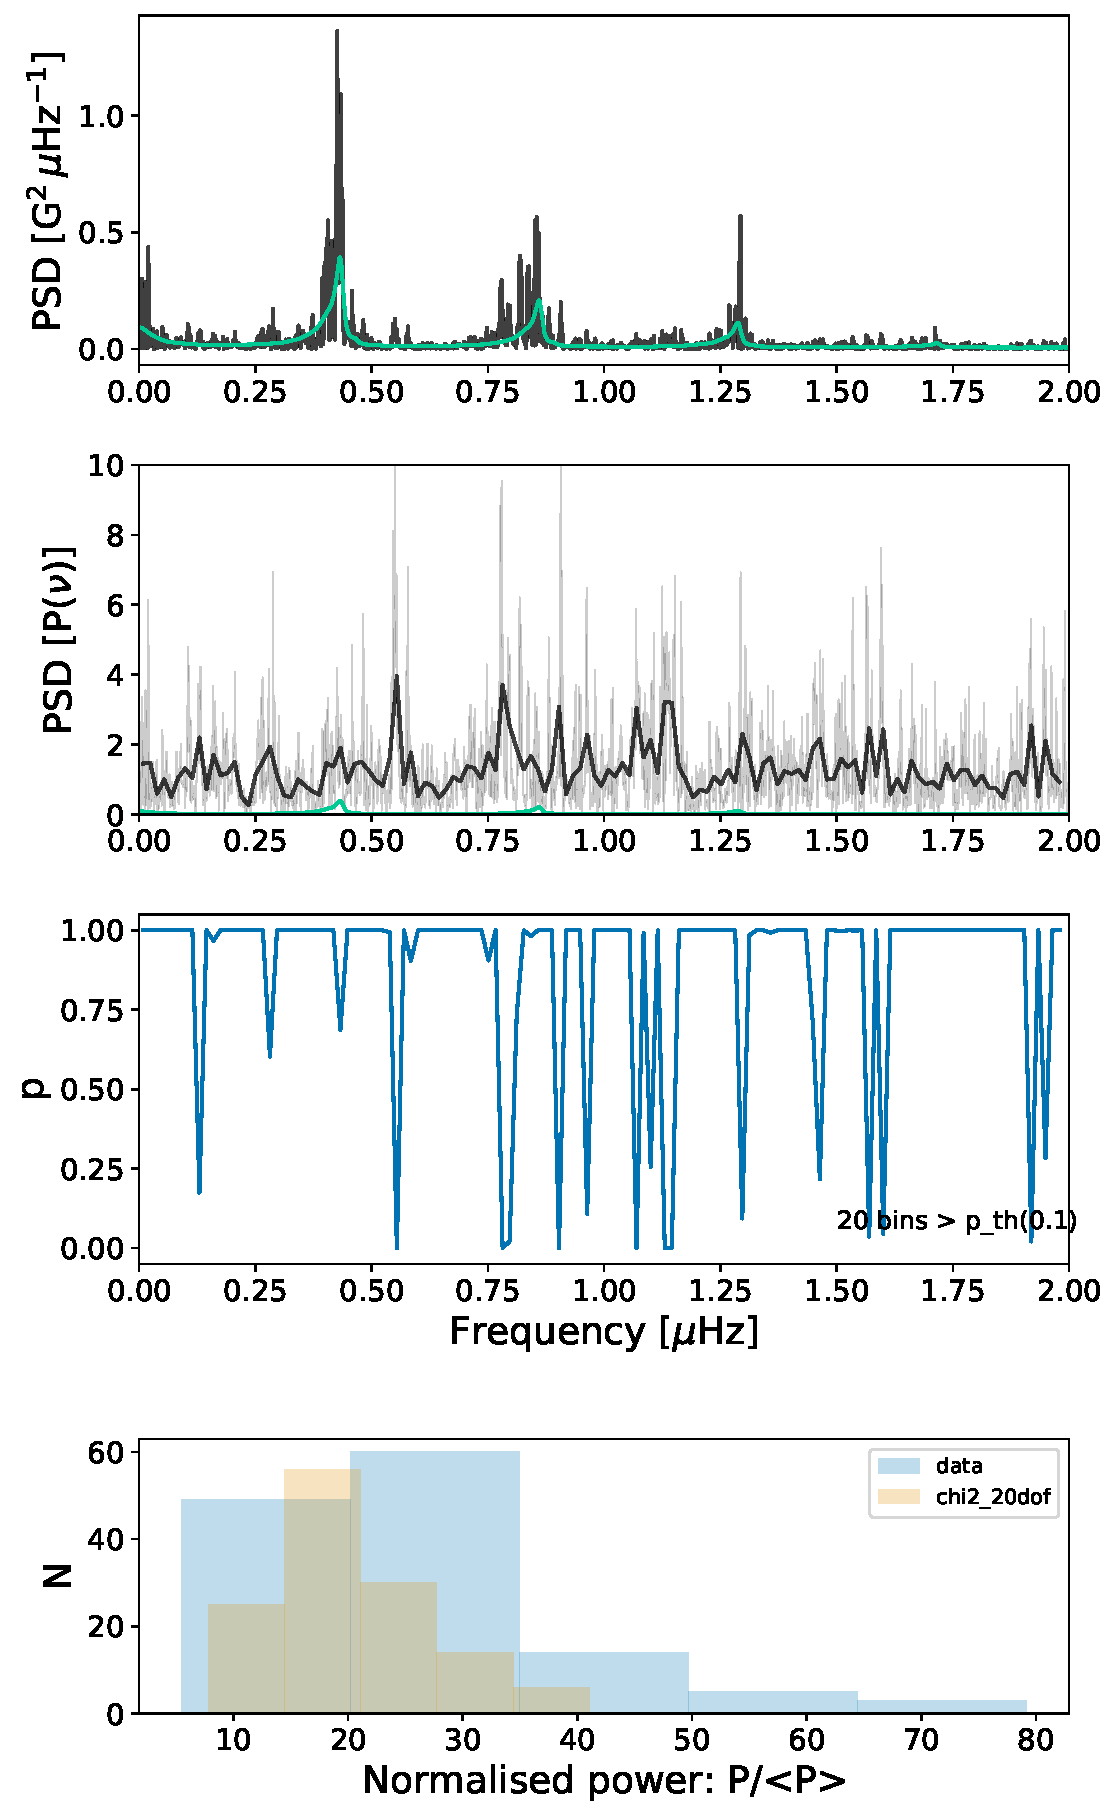
\includegraphics[width=0.35\columnwidth]{full_stats_BiSON_asymm_n10.pdf}
		\label{fig:BiSON_new_asymm_stats_n10}}
	
	\caption{Realisations of the statistics tests on the BiSON data for different re-binning factors (n). The panels of each sub figure are: (top) the full PSD and fit, (second panel) the full and re-binned residuals, (third panel) the probability of statistical noise in each bin, (bottom) distribution of the residuals compared to a $\chi^2$ 2n-DOF.}
	\label{fig:BiSON_new_asymm_stats}
\end{figure}


These tests suggest that the feature around 0.5~$\mu$Hz may be a signal related to $r$ modes, as its location is roughly correct for the $l=m=2$ mode consistently has a low \gls{fa} probability. %The other low \gls{fa} probability features tend to be associated with the residuals from the main harmonics of the \gls{smmf} signal, and are the result of a slight failing of the main model of the power spectrum.
In Figure~\ref{fig:BiSON_new_asymm_stats_n2}, there is compelling evidence to suggest that this feature is significant, in particular. In order to solidify this conjecture, we aimed to fit a model to the residuals around this peak in order to confirm whether the properties of the peak resembled those suggested by \citet{loptien_global-scale_2018}, \citet{liang_time-distance_2019}, and \citet{lanza_sectoral_2019}.


\subsection{Modelling {\it r} mode Profiles}

Using the model for the Lorentzian peak (eq.~\ref{eq:lorentzian}), we modelled the residual spectrum around the location of the potential  $l=m=2$ mode. The results of the fit are given in Table \ref{tab:rmode_fit_params} and the fit to the residuals is shown in Figure \ref{fig:rmode_asymm_fit}.

\begin{table}[!ht]
	\begin{center}
		\caption{Median posterior values of the Lorentzian model for the $r$ mode peak in the BiSON SMMF PSD residuals. Numbers in brackets denote uncertainties on the last 2 digits, and all uncertainties correspond to the 68\% credible intervals either side of the median.}
		\label{tab:rmode_fit_params}
		\begin{tabular}{l c r}
			\hline
			{Parameter} & {Value} & {Unit} \\
			\hline
			
			{$\nu_0$} & {0.5500$\left(_{-16}^{+16}\right)$} & {$\mu\mathrm{Hz} $}\\
			
			{$\Gamma$} & {0.0058$\left(_{-28}^{+45}\right)$} & {$\mu\mathrm{Hz} $} \\
			
			{$A$} & {0.261$_{-0.049}^{+0.063}$} & {--} \\
			
			
			{$bgnd$} & {1.00$\pm 0.16$} & {--} \\	
			
			\hline
		\end{tabular}
	\end{center}
\end{table}

\begin{figure}[!ht]
	\centering
	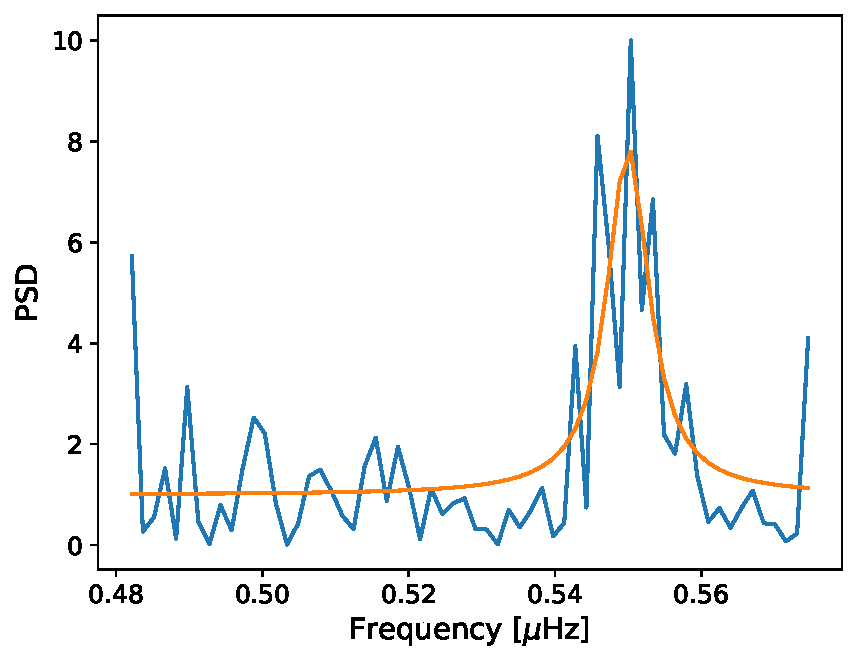
\includegraphics[width=0.65\columnwidth]{asymm_r-mode_model_fit.pdf}
	\caption{Model fit to the $r$ mode in the BiSON PSD residuals using the median from the parameter posterior distributions.}  \label{fig:rmode_asymm_fit}
\end{figure}

The median of the posterior distribution for the width parameter suggests an e-folding lifetime ($1/(\pi \Gamma)$) of around 650 days ($\sim 1.8$ years), which follows the order of magnitude of the lifetime predicted and observed for low-$m$ Rossby modes. The lowest $r$ mode observed, $l=m=3$, was shown to exhibit a lifetime of over a year ($\sim 1.4$ years) by \citet{liang_time-distance_2019}. The $l=m=4$ were observed by both \citet{loptien_global-scale_2018} and \citet{liang_time-distance_2019} to have a lifetime of $\sim 0.6$ years and $\sim 0.3$ years, respectively. There seems to be a slight increasing trend in the mode lifetimes observed by \citet{loptien_global-scale_2018} and \citet{liang_time-distance_2019} of longer lifetimes for lower $m$, therefore the long lifetime found here for the $l=m=2$ mode is entirely reasonable and in-line with current observations.

The model of the mode in the residuals spectrum has a magnetic amplitude of $\sim 30$ mG, which equates to a radial velocity amplitude of $\sim 8.7 \, \mathrm{cm}^{-1}$. \citet{lanza_sectoral_2019} state that the maximum RV amplitude of the $l=m=2$ mode is $\sim 24.5 \,\mathrm{cm}^{-1}$, meaning our observed peak is around a third of the maximum RV amplitude one might have expected to observe. This is however an upper limit given by \citet{lanza_sectoral_2019}, and therefore the lower amplitude in the model should not be concerning.

In particular, however, we can see that the background is $\sim 1$, which is expected for such a fit to residual \gls{psd} data. Due to the accuracy of the background, the agreement between the central frequency of the fit to the $l=m=2$ mode, the agreement in the order of magnitude of the e-folding lifetime, and the amplitude of the mode residing below the upper limit suggested by \citet{lanza_sectoral_2019}, there is evidence to suggest that this peak, which has shown to be significant through the false-alarm statistics tests, could be the $l=m=2$ sectoral $r$ mode, observed in the \gls{bison} \gls{smmf} data. We will cross-check this by further investigation using simulated data and, more directly, by comparison to other sources of \gls{smmf} observations, to determine whether the signal is present there too.







%%%%%%%%%%%%%%%%%%%%%%%%%%%%%%%%%%%%%%%%%%%%%%%%%%%%%%%%%%%%%%%%%%%%%
%%%%%%%%%%%%%%%%%%%%%%%%%%%%%%%%%%%%%%%%%%%%%%%%%%%%%%%%%%%%%%%%%%%%%
\section{Discussion}\label{sec:r-mode_discussion}


Despite the results presented in the previous section there remained an open question on the way the Rossby waves would manifest themselves in the power spectrum. The \gls{bison} power spectrum was also compared to the power spectra of the \gls{wso} \gls{smmf} and the \gls{sdo/hmi} \gls{smmf} to cross-reference the finding.

\subsection{Manifestation of Rossby Waves in the Power Spectrum}

It was suggested by \citet{lanza_sectoral_2019} that the mode should be split into two frequencies due to the annual variation of the B$_0$ angle, but the observed peak in the \gls{bison} spectrum is located at approximately the location of the central frequency and is not split into significant peaks, separated by the predicted separation, due to this modulation. We needed to determine if this was physically observable.

Figure \ref{fig:l2m2} shows a schematic diagram of the flow of a $l=2=m$ sectoral $r$ mode. One can clearly see from the more visible purple region of the schematic, the Southern Hemisphere flow is oriented out of the page, whereas the Northern Hemisphere flow is oriented into the page. Due to the B$_0$ modulation, a varying of the sign of the flow would be observed over this region, i.e the velocity of the flow. In the more red-green regions the schematic, the flow is more transverse, hence this would contribute less to the effect of the B$_0$ modulation.

We needed to therefore understand whether the \gls{smmf} observations have a hemispheric dependence that would lead to a change sign in the observations due to the B$_0$ variation. In addition, this raised the question of how the mode was affected in the power spectrum by the B$_0$ modulation; either split into separate peaks as suggested by \citet{lanza_sectoral_2019} or instead was it possible that we could have a situation where the mode at the central frequency remained?

\begin{figure}[!ht]
	\centering
	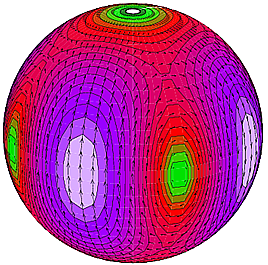
\includegraphics[scale=0.7]{l2m2.png}
	\caption{Mode displacement schematic for an $l=m=2$ $r$ mode \citep{strohmayer_neutron_2014}}  \label{fig:l2m2}
\end{figure}

To investigate the splitting of the mode, a simple model was produced whereby a sinusoidal function (with a period of $\sim$25 days) was modulated by either a cosine or rectified cosine function (with a period of 1 year). In the former, using the cosine modulation, this represents observing the sign of the flow varying with the B$_0$ modulation. Conversely in the latter simulation, this instead represents a variation of the amplitude, and it does not change the sign. Figure \ref{fig:modulation} shows the time series of the two cases to more clearly show their difference. The power spectrum of each case was then computed and these are shown in Figure \ref{fig:modulation_PSDs} to demonstrate the differences between the modes produced.

\begin{figure}[!ht]
	\centering
	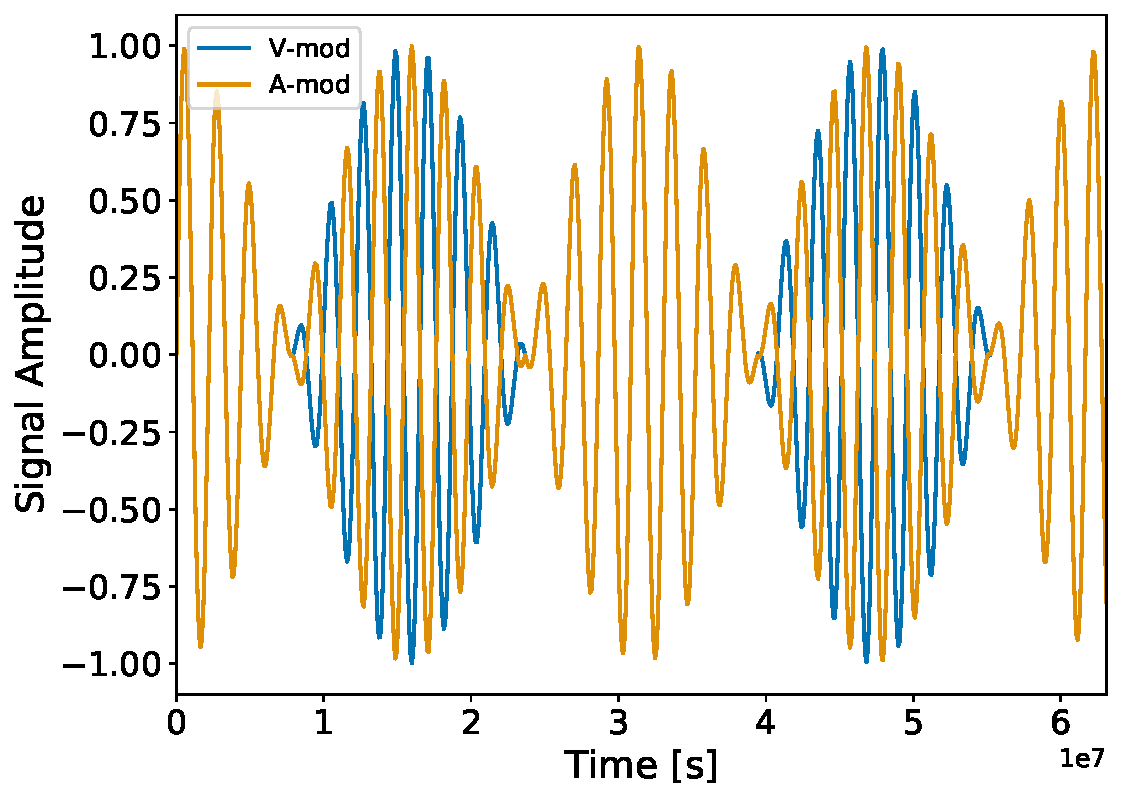
\includegraphics[width=0.65\columnwidth]{modulation_plot.pdf}
	\caption{Time series of the velocity and amplitude modulation toy model simulations. The blue curve shows the velocity modulation, i.e. modulating using a cosine with period of 1 year, whereas the orange curve shows the amplitude modulation, i.e. modulating using a rectified cosine with period 1 year.}  \label{fig:modulation}
\end{figure}

\begin{figure}[!ht]
	\centering
	\subfloat[Velocity modulation]
	{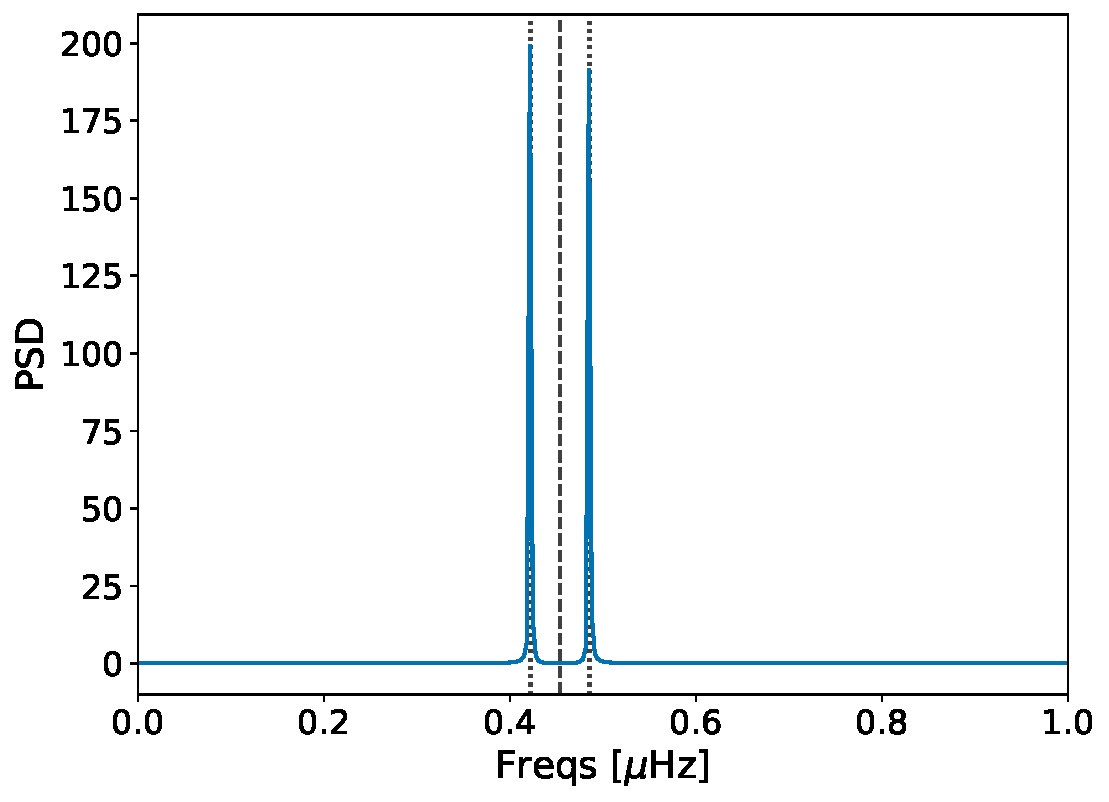
\includegraphics[width=0.47\columnwidth]{v_mod.pdf}} 
	\qquad
	\subfloat[Amplitude modulation]{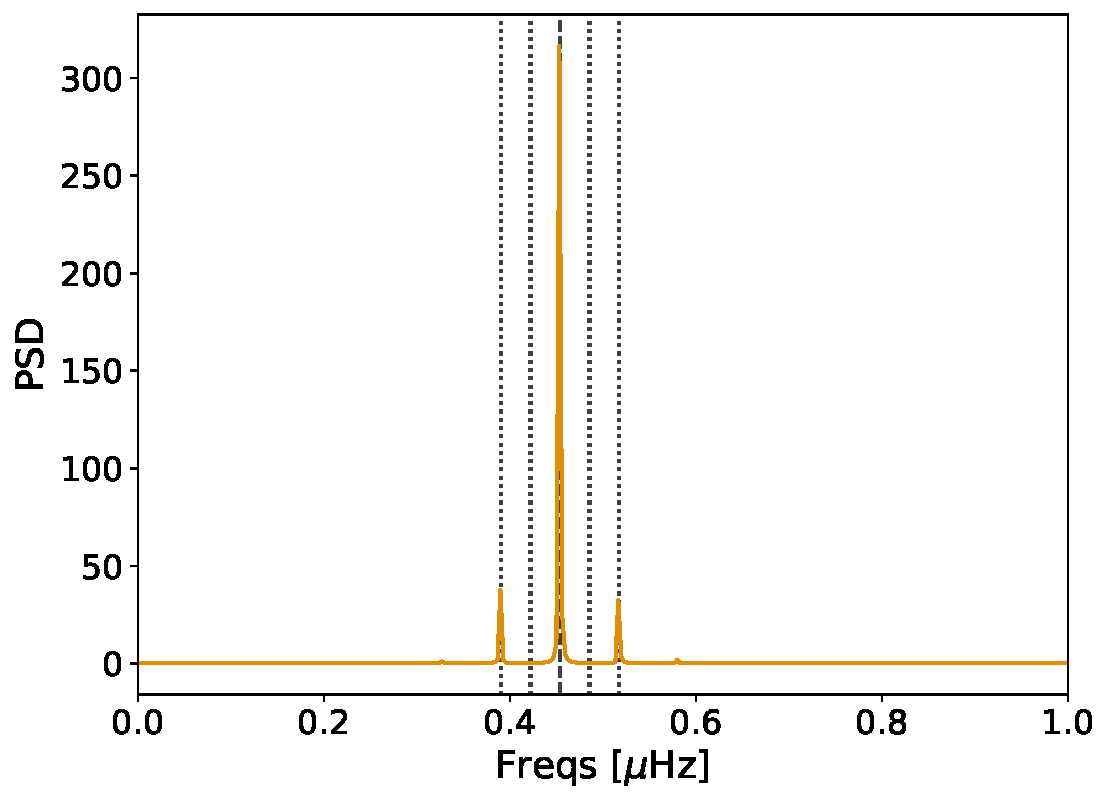
\includegraphics[width=0.47\columnwidth]{a_mod.pdf}}
	\caption{Power spectra for the two modulation methods, showing the difference in the way the modulation has changed the frequency of the observed mode.}  \label{fig:modulation_PSDs}
\end{figure}

One can clearly see the difference in the power spectrum produced in each of the cases. In the velocity modulation case, we see a splitting of the oscillation mode into two peaks split around the expected mode frequency by $\pm \nu_{\oplus}$. There exists no more power at the central mode frequency in this case and is in agreement with the scenario suggested by \citet{lanza_sectoral_2019}. In the amplitude modulation case, we see sidebands at $\pm 2\nu_{\oplus}$ however the expected mode frequency remains in this scenario and has a significantly higher peak height, a ratio of ~90:10 in favour of the central peak.

We have shown that it is possible to retain the central frequency of the $r$ mode in the power spectrum  if the B$_0$ modulates the amplitude of the observations and not the sign. With this known, it was then necessary to understand whether the two hemispheres of the Sun contribute signals that are more analogous with the velocity modulation or amplitude modulation. In the former, velocity modulation, we would expect to see a persistent anti-correlation between the two hemispheres. In the latter, amplitude modulation, we would expect to see the signals from each hemisphere that are correlated, which track each other and which can be both positive or negative.

We investigated how the two hemispheres of the Sun contribute to the \gls{smmf} through analysis of \gls{sdo/hmi} data. To do this, we acquired 720s-cadence magnetograms from \gls{sdo/hmi} using the {\verb SunPy } python module \citep{barnes_sunpy_2020} for the rising phase of solar cycle 24 during 2011, and for the maximum of cycle 24 during 2014. It was possible to separately average the Northern and Southern Hemispheres' contributions to the total, disk-averaged \gls{smmf}. The plot of this data is shown in Figure~\ref{fig:HMI_MF}.

\begin{figure}[!ht]
	\centering
	\subfloat[2011]
	{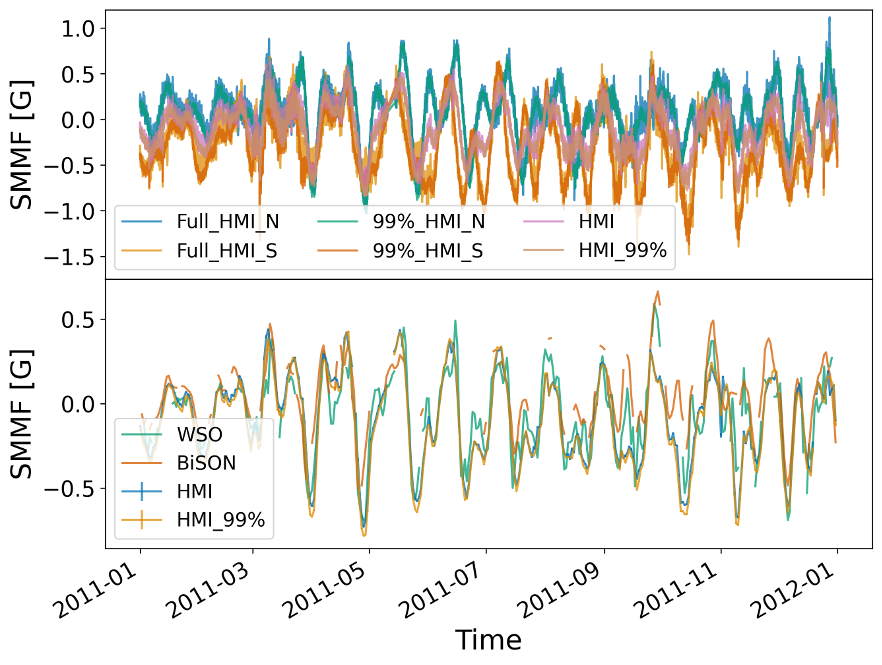
\includegraphics[width=0.47\columnwidth]{HMI_MF_2011_rescaled.png}} 
	\qquad
	\subfloat[2014]{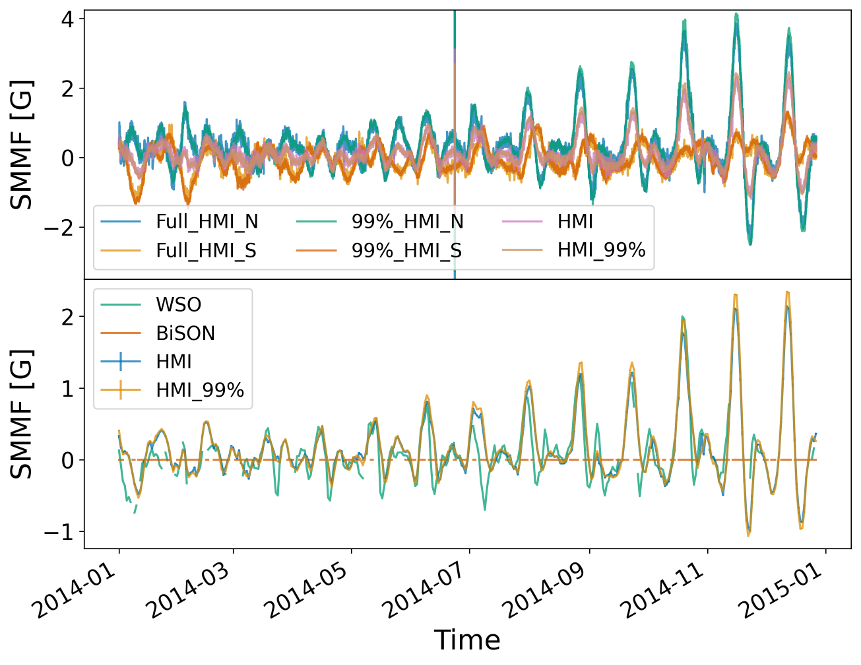
\includegraphics[width=0.47\columnwidth]{HMI_MF_2014_rescaled.png}}
	\caption{SDO/HMI SMMF split into hemispheres and compared to other SMMF sources during (a) 2011, and (b) 2014. The top panel in each figure shows the north (N), south (S), and total disk-averaged mean magnetic field, for both the full solar disk and from pixels within 99\% of solar radius. The bottom panels show a comparison between the SMMF, as observed BiSON, WSO, and SDO/HMI (full disk and the 99\% disk).}  \label{fig:HMI_MF}
\end{figure}


The hemispheric contributions to the total, disk-averaged, \gls{smmf} can be seen in Figure~\ref{fig:HMI_MF} to track each other during 2011, and both become positive or negative. By contrast, when observing the hemispheric contributions to the full \gls{smmf} in 2014, we see that there are frequent periods of strong anti-correlation between the Northern and Southern Hemispheres. There are also several periods in 2014 whereby the two hemispheres are correlated. This plot aids in our understanding of how the $r$ modes would be manifested in the power spectrum due to the variation of the B$_0$ angle. 

As there are periods of both strong correlation and strong anti-correlation between the two hemispheres, this is a good indication that the $r$ mode signal would result in a central frequency with sidebands due to the correlation between North and South. But due to the existence pf periods of anti-correlation between North and South, we also expect there to be some degree of frequency splitting in the power spectrum, but this is dependent on how prevalent the anti-correlation is over the entire solar cycle; in these short epochs however, we expect this to be minimal. It is therefore possible to conclude that we are confident we are observing the $l=2=m$ $r$ mode.

As a further point, we see that there is both strong correlation and strong anti-correlation between the Northern and Southern Hemispheres, however this does not necessarily mean that the $r$ mode signal would directly manifest itself in the same way. We can see from Figure~\ref{fig:l2m2} that if the $r$ mode observations are constrained to active latitude bands, closer to the equator, then the effects of the B$_0$ are less prominent.

\subsection{Rossby Modes in Other Sources of SMMF Data}

To further investigate whether the observation of the  $l=2=m$ $r$ mode is real, a comparison was made between the power spectrum of the \gls{bison} observations of the \gls{smmf} and those from \gls{wso} and \gls{sdo/hmi}, to determine whether the suspected $r$ mode is visible. In the case of the \gls{wso}, the power spectrum was computed over the same observing epoch as the \gls{bison} data (i.e. from 1992 -- 2013); however SDO was not launched until 2010, so for HMI the power spectrum was computed on data from 2010 -- 2020, hence at approximately half the frequency resolution of \gls{wso} and \gls{bison}.

Figure~\ref{fig:comparing_SMMF_PSDs} shows the comparison of the \gls{wso} and \gls{sdo/hmi} power spectra reflected around the x-axis against the \gls{bison} power spectrum. In both cases we see a good agreement between the different sets of data on the location of the rotational mode in the \gls{smmf}, but there does not appear to be a visible $r$ mode candidate in the \gls{wso} or the \gls{sdo/hmi} data.

\begin{figure}[!ht]
	\centering
	\subfloat[WSO]{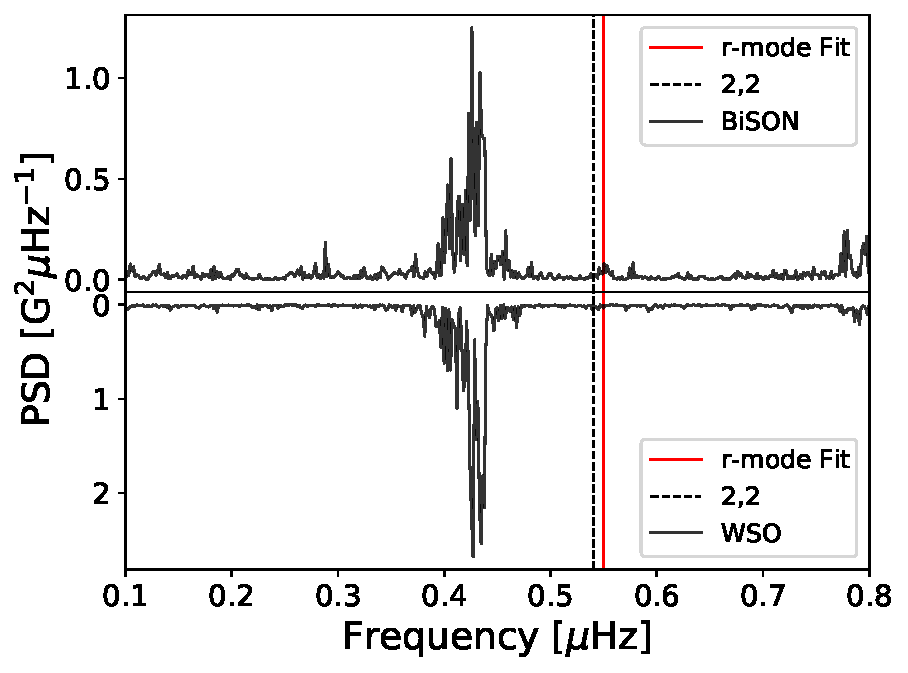
\includegraphics[width=0.47\columnwidth]{BiSON_vs_WSO_r-mode.pdf}} 
	\qquad
	\subfloat[HMI]{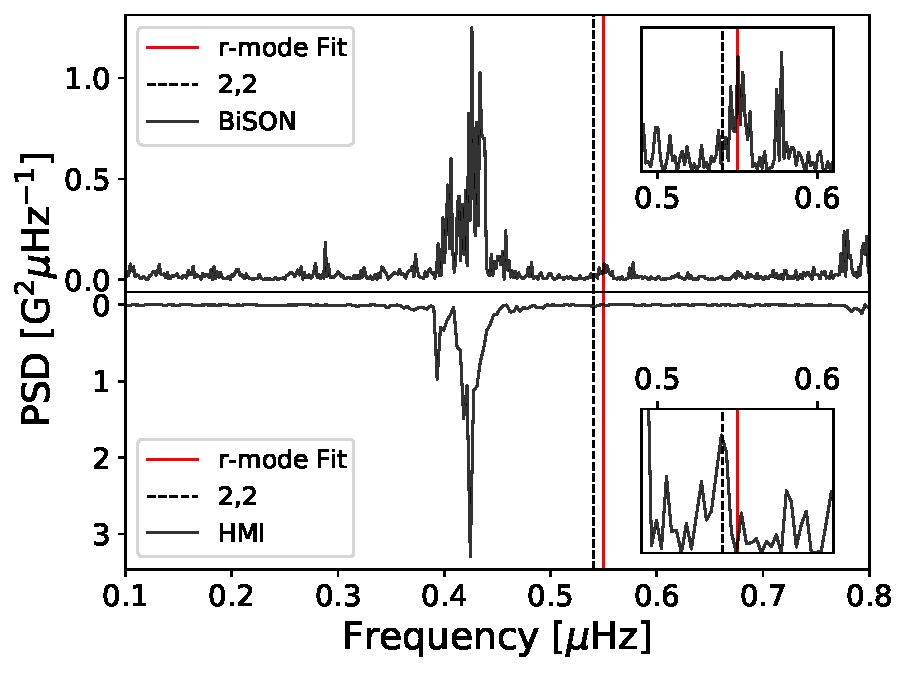
\includegraphics[width=0.47\columnwidth]{BiSON_vs_HMI_r-mode.pdf}}
	\caption{Comparison of the power spectra for BiSON, WSO, and SDO/HMI. In both figures, the top panel shows the BiSON PSD and the bottom panel shows either the WSO or HMI PSD. The dashed, black line shows the location of the theoretical $l=2=m$ $r$ mode frequency, and the red, solid line shows the location of the peak fit in the BiSON PSD residuals.}  \label{fig:comparing_SMMF_PSDs}
\end{figure}

This provides concerning evidence that we may not, in fact, have observed the $l=2=m$ $r$ mode in the \gls{bison} power spectrum, and perhaps instead we have a persistent noise source in the \gls{bison} \gls{smmf}.

However compelling the results are, suggesting that we may have observed the $l=2=m$ $r$ mode in the \gls{bison} power spectrum, it is impossible to ignore that it is not present in two other sources of \gls{smmf} observations -- of which one of these telescopes is responsible for providing the recent observations of $r$ modes documented in the literature (\gls{sdo/hmi}). Owing to this, we cannot conclude that we have observed the $l=2=m$ $r$ mode in the \gls{bison} power spectrum. We recommend that searching for $r$ modes in the power spectra of the \gls{smmf} observations should be revisited in a few years, or say a solar cycle's time, when the frequency resolution in each power spectrum has increased significantly, to provide a more insightful follow-up study.


%%%%%%%%%%%%%%%%%%%%%%%%%%%%%%%%%%%%%%%%%%%%%%%%%%%%%%%%%%%%%%%%%%%%%
%%%%%%%%%%%%%%%%%%%%%%%%%%%%%%%%%%%%%%%%%%%%%%%%%%%%%%%%%%%%%%%%%%%%%
\section{Conclusion}\label{sec:r-mode_conclusion}

After removing the model for the \gls{bison} \gls{smmf} power spectrum we investigated the residual spectrum to search for the existence of Rossby wave modes ($r$ modes). Using a false-alarm approach we estimated the probability of finding narrow-band power. We identified the existence of a statistically significant peak which was near the $l=2=m$ $r$ mode frequency calculated by \citet{lanza_sectoral_2019}.

Using a Lorentzian model for the peak, following the description of $r$ mode given by \citet{loptien_global-scale_2018} and \citet{liang_time-distance_2019}, we identified the properties of the peak, and compared them to the existing literature. The work by \citet{lanza_sectoral_2019} stated that the $l=2=m$ $r$ mode should be observed at a frequency of $\sim 540.8$ nHz, with a maximum amplitude of $24.5 \, \mathrm{cm}^{-1}$. The recent observations of low-degree sectoral $r$ modes by \citet{loptien_global-scale_2018} and \citet{liang_time-distance_2019} claimed the line-width of the mode would be on the order of around 10 nHz, due to the e-folding lifetime of the mode being on the order of a year.

To further interrogate the inferences on the $r$ mode in the \gls{bison} \gls{smmf} power spectrum, we use simple simulations to determine how the $r$ mode may manifest itself in the power spectrum, using the modulation of the signal due to the variation in the B$_0$ angle. Furthermore, \gls{sdo/hmi} hemispheric data were employed to verify these results.

As a final check, we compared the power spectrum of the \gls{smmf} observations from \gls{bison} to those from \gls{wso} and \gls{sdo/hmi}. There was no clear signature of the $l=2=m$ $r$ mode in either of the other power spectra, which rules our observation of an $r$ mode in the \gls{bison} \gls{smmf} very suspicious, especially as the recent observations of sectoral Rossby waves in the Sun have all used \gls{sdo/hmi} data.

We leave the reader with the following points:

\begin{enumerate}
	\item{Through a series of false-alarm probabilty statistical tests, we have shown that there exists a statistically significant peak in the \gls{bison} \gls{smmf} residuals spectrum which is located near the theoretical frequency of the $l=2=m$ $r$ mode.}
	
	\item{By modelling the peak as a Lorentzian profile we find that the peak has a central frequency of $550 \pm 16$ nHz (i.e. located $\sim 9.2$ nHz from the theoretical frequency), a line-width of $5.8^{+4.5}_{-2.8}$ nHz, and an amplitude of $\sim 30$ mG. This profile is within the upper limit for the amplitude of the $l=2=m$ $r$ mode and the life time implied by the line-width is on the order of 1--2 years, which is in agreement with the observations by \citet{loptien_global-scale_2018} and \citet{liang_time-distance_2019}.}
	
	\item{Through the analysis of simulated data and hemispheric observations of the \gls{smmf}, we have shown that we should expect to see a prominent mode at the theoretical frequency, and not a split mode due to the effect of the B$_0$ variation, which supported the findings of the $r$ mode.}
	
	\item{By comparing the power spectrum of the \gls{smmf} observed by \gls{bison}, to those of \gls{wso} and \gls{sdo/hmi}, we have shown that the $r$ mode peak is not manifested in either the \gls{wso} or \gls{sdo/hmi} spectra, therefore ruling it highly unlikely that the observed peak in the \gls{bison} spectrum is the $l=2=m$ $r$ mode.}
\end{enumerate}


As we collect more observations of the \gls{smmf} using \gls{bison}, the frequency resolution of the power spectrum increases. An obvious next step in this work is to collect more observations of the \gls{smmf} with \gls{bison}, to further investigate if this suspected mode remains resolved, or whether it diminishes into the noise.